\documentclass[UTF8, 12pt, A4paper]{article}



% ---- 导言区 ----

% -- 表格美化相关包 --
\usepackage{tcolorbox}
\usepackage{array,tabularx}
\usepackage{colortbl}
% -- 表格美化相关包 --

\usepackage{xeCJK}  % 中文
\usepackage{fancyhdr} % 页眉页脚
\usepackage[left=2cm, right=2cm, top=2.5cm, bottom=3cm]{geometry} % 页边距
\usepackage{graphicx} % 插入图片
\usepackage{xcolor} % 设置16色字体颜色时需要
\usepackage[colorlinks, linkcolor=blue]{hyperref} % 超链接,可改链接颜色
\usepackage{indentfirst} % 每节首个段落缩进
\usepackage{listings} % 插入代码块
\usepackage{fontspec} % 代码块选字体
\usepackage{amssymb} % 数学符号
\usepackage{newverbs} % 行内代码高亮
\usepackage[perpage]{footmisc} % 防止脚注编号不够的包
\usepackage{ulem} % 删除线的包
\usepackage{xpinyin} % 拼音的包

% 非常重要,新版本的BibLaTeX默认使用Biber而非BibTeX进行处理参考文献。不设置这个的话,目录会出不来。
\usepackage[backend=bibtex]{biblatex} 




% ---- 基本设置区 ----
% 设定页面的页眉页脚类型,$\LaTeX$内置了四种:empty、plain、headings及myheadings,但是我们现在不用这些内置的样式。
\pagestyle{fancy}
% 清除原页眉页脚样式
\fancyhf{} 
% 设置页眉 备注:O代表odd(奇数页),E代表even(偶数页)
\fancyhead[LO, LE]{
    \begin{minipage}[c]{0.06\textwidth}
		
\includegraphics[height=7.5mm]{PMU-SEF-logo.pdf}
	\end{minipage}} % 左页眉
% \fancyhead[RO, RE]{右页眉} % 右页眉
% 设置页脚
\fancyfoot[LO, LE]{\textcolor[HTML]{BEBEBE}{\copyright 贝石拌饭}} % 左页脚
% \fancyfoot[RO, RE]{\leftmark} % 右页脚
\fancyfoot[RO, RE]{
    \begin{minipage}[c]{0.06\textwidth}
		
\includegraphics[height=12.5mm]{emergency-food.png}
	\end{minipage}} 
\fancyfoot[CO, CE]{\thepage} % 中页脚
% 页眉线宽,设为0可以去页眉线
\renewcommand{\headrulewidth}{0.2mm} 
% 页脚线宽,设为0可以去页眉线
\renewcommand{\footrulewidth}{0mm} 

% 字体
\setCJKsansfont{Source Han Sans CN} % 思源黑体
% \setCJKmonofont{Sarasa Gothic CL} % 更纱黑体
\setmonofont{Consolas}
\setCJKmainfont[BoldFont=SimHei,ItalicFont=KaiTi]{Source Han Sans CN} % 不弄这个引用文献可能会出错。

% 在section前加入§符号的功能设置(不需要导入包)
\makeatletter
%% See pp. 26f. of 'The LaTeX Companion,' 2nd. ed.
\def\@seccntformat#1{\@ifundefined{#1@cntformat}%
    {\csname the#1\endcsname\quad}%      default
    {\csname #1@cntformat\endcsname}}%   individual control
\newcommand{\section@cntformat}{\S\thesection\quad}
% \newcommand{\subsection@cntformat}{\S\thesubsection\quad}
% \newcommand{\subsubsection@cntformat}{\S\thesubsubsection\quad}
% \newcommand{\paragraph@cntformat}{\S\theparagraph\quad}
% \newcommand{\subparagraph@cntformat}{\S\thesubparagraph\quad}
\makeatletter

% 将作者脚注文本那边的标号也设为特殊符号,不然为数字
\renewcommand{\thefootnote}{\fnsymbol{footnote}}

% 代码块区域设置
\definecolor{mygreen}{rgb}{0,0.6,0}
\definecolor{mygray}{rgb}{0.5,0.5,0.5}
\definecolor{mymauve}{rgb}{0.58,0,0.82}
\lstset{ %
backgroundcolor=\color[RGB]{245,245,244},       % choose the background color
basicstyle=\footnotesize\ttfamily,              % size of fonts used for the code
columns=fullflexible,
breaklines=true,                                % automatic line breaking only at whitespace
captionpos=b,                                   % sets the caption-position to bottom
tabsize=4,
commentstyle=\color{gray},                      % 注释样式
escapeinside={\%*}{*)},                         % if you want to add LaTeX within your code
keywordstyle=\color{magenta},                   % 关键词样式
stringstyle=\color{mymauve}\ttfamily,           % string literal style
frame=single,
rulesepcolor=\color{blue!20!green!20!blue!20},
% identifierstyle=\color{red},
language=python,
numbers=left,                                        % 在左侧显示行号
numberstyle=\tiny\color{gray}\ttfamily,              % 设定行号格式
}

% 表格颜色等格式设置
\tcbuselibrary{skins}

\newcolumntype{Y}{>{\centering\arraybackslash}X} % 表格文字居中

\tcbset{tab2/.style={enhanced,fonttitle=\bfseries,fontupper=\normalsize\sffamily,
colback=yellow!10!white,colframe=red!50!black,colbacktitle=pink!40!white,
coltitle=black,center title}} % 表格颜色与其他格式设置

% 行内代码高亮命令,自定义cverb命令,不高亮还是verb命令
\newverbcommand{\cverb}{\color{red}}{}

% Using symbols for footnotes
\renewcommand{\thefootnote}{\fnsymbol{footnote}}












% ---- 封面区 ----
\title{
    
\includegraphics[scale=1]{PMU-logo.pdf} \\ % 封面标题前加图片
    ~\\
    派蒙也能看懂的中国狐意象考据整理
    }
\author{贝石拌饭\footnotemark[1] \footnotemark[2]}
\date{创建:December 17, 2021 || 更新:\today}
\linespread{1.5}



% ---- 正文区 ----
\begin{document}

% 第一页:封面
\maketitle
\footnotetext[1]{Homepage: \url{https://www.zhihu.com/column/CLKuma}} % 作者脚注
\footnotetext[2]{E-Mail: kaede0614@126.com}
\thispagestyle{empty} % 清空封面页的格式

\textbf{说明:}派蒙,最好的应急食品!


\begin{figure}[ht]
    \centering
    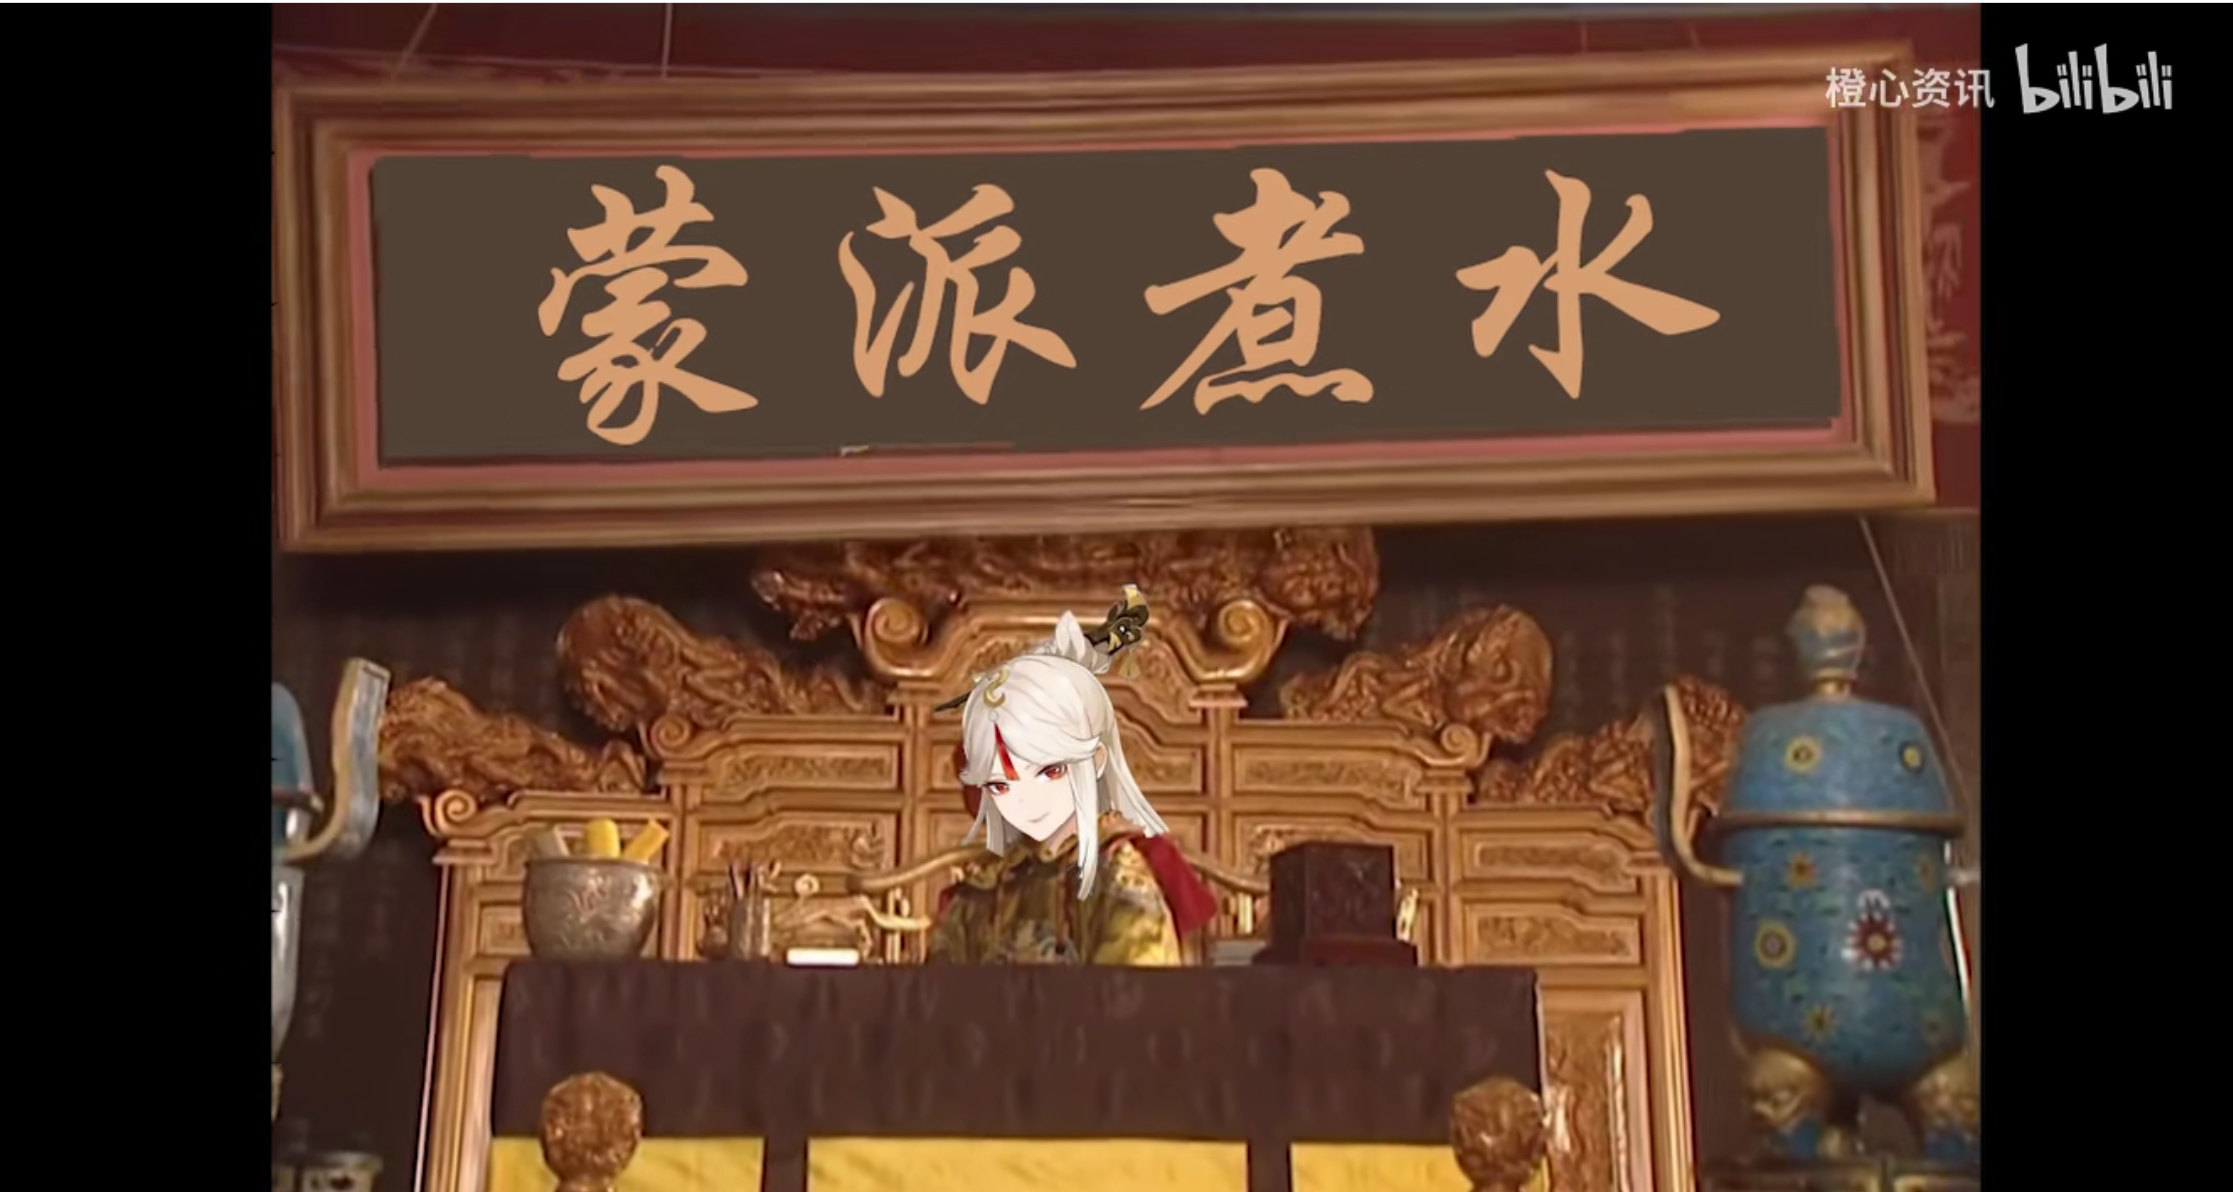
\includegraphics[width=15cm]{蒙派煮水.png}
\end{figure}


% 第二页:目录
\newpage
% 添加目录
\pagenumbering{roman} % 页码数字显示风格
\setcounter{page}{1} % 页码编号手动设置
\tableofcontents

% 正文
\newpage
\setcounter{page}{1}
\pagenumbering{arabic}

% section
\newpage
\section{我国狐意象的发展脉络}

\subsection{上古——狐图腾与狐姓氏}

最早的史籍对狐的记载寥寥无几,《古本竹书纪年》记载第七任夏王\xpinyin*{杼}东征达到东海和王寿(或称三寿),得到一只九尾狐\footnote{《古本竹书纪年》:“柏杼子征于东海及三寿 , 得一狐九尾 。”}。《周易》记载田野间捕获了三只狐狸\footnote{《周易》解卦九二爻辞:“田获三狐,得黄矢。贞吉。”}。其他关于狐的意象是“狐死首丘”的典故,即狐狸死在外面一定会把头朝向洞穴的方向,《礼记·檀弓》\footnote{《礼记·檀弓》:“古之人有言曰:‘狐死正丘首,仁也。’”}和《九章·哀郢》\footnote{《九章·哀郢》 :“鸟飞反故乡兮 , 狐死必首丘 。”}均有记载 。


\subsubsection{青丘之狐与太皞伏羲氏}

上古史有很多不可考的东西,下面讲的只是我个人整理出觉得比较有趣的说法,不是正经研究,不可作为证据。

狐在古籍中最早记载于《山海经》,其中《大荒东经》\footnote{《山海经·大荒东经》“有青丘之国 ,有狐,九尾。” }、《海外东经》\footnote{《山海经·海外东经》:“青丘国在其北,其狐四足九尾。”}、《东山经》\footnote{《山海经·东山经》:“有兽焉,其状如狐而九尾、九首、虎爪,名曰蠪蛭,其音如婴儿,是食人。”}、《南山经》\footnote{《山海经·南山经》:“又东三百里,曰青丘之山,其阳多玉,其阴多青雘。有兽焉,其状如狐而九尾,其音如婴儿,能食人,食之不蛊。”}中出现的狐均为九尾,且提到了“青丘”这个地名,说明九尾狐出于青丘,那么青丘在哪呢?注意上面记载了九尾狐的四卷,三卷为东。中原的东边是东夷文化区,而东夷最古老是太皞部系,后来和伏羲氏合并称为太皞伏羲氏,为风姓\footnote{《古本竹书纪年》:“太皞伏羲氏,以木德王,为风姓。”}\footnote{《春秋左氏传·僖公二十一年》:“任、宿、须句、颛臾,风姓也。”},对没错,伏羲和女娲其实都是风姓。西晋皇甫\xpinyin*{谧}著《帝王世纪》记载太皞伏羲的母亲华胥在雷泽看到一个巨大的脚印,走了一趟就怀孕生下伏羲\footnote{《帝王世纪》:“有巨人迹出于雷泽,华胥以足履之,有娠,生伏羲于成纪。”}。那么风姓和青丘有什么关系呢?西汉东方朔著《十洲记》记载,长洲又叫青丘,青丘有风山,山中常年有雷声\footnote{《十洲记》:“长洲又名青丘,在南海辰巳之地。地方各五千里,去岸二十五万里。上饶山川及多大树,树乃有二千围者。一洲之上,专是林木,故一名青丘。又有仙草灵药,甘液玉英,靡所不有。又有风山,山恒震声。有紫府宫,天真仙女游于此地。”}。风山常年有雷声,风姓华胥履雷泽,故事这就扣上了,青丘基本可以认为是太皞伏羲氏的故地。既然九尾狐出于青丘,能否认为九尾狐或者雷在太皞伏羲氏的东夷部落中有特殊意义?无法确定,上古的东西基本都是不可考的。实际上面说的故事有一团的问题,比如太皞伏羲是否是同一人,伏羲是否是东夷人,风姓一开始是哪边的,雷泽的雷神和华胥是否有关系,燧人氏和雷神是否是同一人等等。既然不可考,这里就先放下了,毕竟本文是谈狐的,接着说。

不可考的太皞伏羲故事告一段落,接着到夏朝的有穷氏首领后羿,《楚辞·离骚》记载后羿喜欢射大狐狸(封狐,有说风狐音转)\footnote{《楚辞·离骚》:“羿淫游以佚畋兮,又好射夫封狐。”}。《淮南子·本经训》又记载后羿在青丘之泽杀“大风” \footnote{《淮南子·本经训》:“缴大风于青邱之泽。”},“大风”多有种说法,如风伯和猛禽,而东夷文化本身就多鸟图腾崇拜,合理推测后羿这次应当是讨伐了太皞后裔的青丘之地风姓部落。接着就是车万狗熟悉的纯狐\xout{妈妈},《楚辞·天问》记载了后羿的妻子纯狐氏与寒浞合谋杀了后羿\footnote{《楚辞·天问》:“浞娶纯狐,眩妻爰谋。”},随后《左传·襄公四年》记载寒\xpinyin*{浞}娶羿妻纯狐氏,生了浇和\xpinyin*{豷}两个儿子\footnote{《左传·襄公四年》:“浞因羿室,生浇及豷”}。纯狐为什么叫纯狐呢?当然是不可考啦。有很多说法,如纯狐和玄妻为同一人,纯狐即黑狐而玄妻指头发秀美乌黑;也有说纯狐氏是以玄狐即黑狐\footnote{闻一多《天问疏证》:“纯玄不惟声近,亦且义同。”}为图腾的氏族。但无论如何,纯狐大概是和狐这个意象有关的,那上古记载中什么和狐密切相关呢?青丘。而后羿可能讨伐过青丘,这不就巧了。后羿伐青丘,妻纯狐谋杀后羿,虽然不可考,但总是让人感觉可疑。

《山海经》所记载的青丘之狐应当是最早的九尾狐意象。虽然基本都是不可考的东西,上面所述的也是有趣的猜测而不是正经论证,但神秘感总是有莫名的吸引力,就像玛奇玛小姐一样。

\subsubsection{涂山之狐与大禹}

涂山之狐意象的出现晚于青丘之狐,最早的记载可能是《楚辞·天问》中的“焉得彼\xpinyin*{嵞}山女,而通之於台桑?”,也有说《尚书·皋陶谟》中有记载\footnote{《尚书·皋陶谟》:“娶于涂山。辛壬癸甲。启呱呱而泣。矛弗子。惟荒度土功。”},但我因为精力原因没找到。另外,东汉赵晔《吴越春秋·越王无余外传》,说大禹30岁了还未婚,在涂山遇到东夷涂山氏之女娇就娶了\footnote{《吴越春秋·越王无余外传》:“禹年三十未娶 , 行涂山 , 恐时之暮, 失其制度, 乃辞曰:‘吾之娶也, 必有应矣。’乃有九尾白狐, 造于禹 。禹曰:‘白者吾之服也。其九尾者, 王者之征也 ……’禹因娶涂山, 谓之女娇 。” }。涂山之狐的典故还诞生了第一首有史可查的情诗,记于《吕氏春秋·音初篇》:“候人兮猗”。另外还有涂山歌,看文献说《吕氏春秋》和《吴越春秋》均有记载,但我暂时没找到。不过涂山歌的狐意象味儿就很浓了:“\xpinyin*{绥}绥白狐,九尾庞庞。成于家室,我都攸昌。”独行的白狐,大以巴毛茸茸,非常可爱的形象。开创家天下的夏朝第二位君主启就是涂山氏和禹的儿子,见于《淮南子》\footnote{《汉书·武帝纪》颜师古注引《淮南子》:“涂山氏往,见禹方作熊,惭而去,至嵩高山下化为石,方生启。禹曰:‘归我子!’石破北方而启生。”}和西汉刘向《列女传》\footnote{《列女传·母仪传·启母涂山》):“启母者,涂山氏长女也。夏禹娶以为妃。”}。可以看出相比于青丘之狐,涂山之狐的相关记载多了颜色特征,即明确为九尾白狐。

相比神秘的青丘之狐,涂山之狐明显多了些暖意,尤其是禹娶妻的爱情故事可能对后世狐意象的变化产生了影响。肯定有人想到了《狐妖小红娘》的涂山一家子,没错,作为爱情故事,为什么叫涂山苏苏而不是青丘苏苏、纯狐苏苏或者风苏苏,制作组大概也有这层考虑吧。

个人找到的涂山狐下一次出现在文献中要到一千多年后的宋代李\xpinyin*{昉}的《太平广记》,记载涂山青狐被献给纣王,因而周文王得以从\xpinyin*{羑}里脱身\footnote{《太平广记·卷四百四十七·狐一》:“周文王拘羑里,散宜生诣涂山,得青狐以献封,免西伯之难。”}。有人说,哎不对,历史上的周文王是被纣王杀了做祭祀,也就是“册”了,肋骨往外翻。这是网络上比较流行的说法,因为听上去比较哈人和猎奇。实际上我翻了翻相关文献,大部分还是倾向于认为“册周方伯”是征讨或册封的意思。因为和狐无关这里就不展开了,想深入的话知网关键词搜“周原甲骨”有一堆相关考证。


再往后个人就没有再找到有关涂山狐的记载,如果有更多资料可以联系封面脚注的邮箱交流。

\subsubsection{妲己与有苏氏}

我是95后,同代人小时候应该大多都看过90版《封神榜》,对于苏妲己的故事应该很清楚,冀州侯苏护的女儿嘛。这里就不再讲些大家都知道的事情,聊点别的。说到苏妲己,大众普遍的第一反应是明代小说《封神演义》,更了解一些的可能会说元代《武王伐纣平话》中苏妲己就是狐狸精了。有人会说,哎不对,妲己最早并没有苏姓,是《国语·晋语》提到纣王伐有苏,有苏氏献女妲己\footnote{《国语·晋语》:“殷辛伐有苏,有苏氏以妲己女焉,妲己有宠,于是乎与胶鬲比而亡殷。”}。问题来了,妲己姓不姓苏呢?当然不是,妲己是有苏氏-己姓的姑娘妲,己才是姓\footnote{《国语·晋语》韦昭注:“有苏,己姓之国,妲己其女也。”}。“苏妲己”本身就是个画蛇添足的叫法,也许因为这个原因,现代作品中“苏妲己”这个名字已经很少出现了,多是直接叫“妲己”,如妖怪名单、武庚纪、妲己不是坏狐狸、鬼灯的冷彻等。

看到这有人会说,封神演义不行啊,妲己的淫恶妖狐形象是不是也元代、明代人编的?虽然妲己很早就作为负面人物出现在史籍中,如《吕氏春秋》\footnote{《吕氏春秋·先识览》:“妲己为政,赏罚无方,不用法式,杀三不辜,民大不服。”}、《史记·殷本纪》\footnote{《史记·殷本纪》:爱妲己, 妲己之言是从。”}和《列女传·\xpinyin*{孽嬖}传》,但并没有狐狸精的形象。严格来说,文学作品中可考的妲己狐狸精形象最早应该就是元人的《武王伐纣平话》。为什么我要加上“严格来说”和“文学作品”这两个定语呢?因为不严格来说,唐代白居易的乐府诗《古冢狐》中已经出现“妖狐”和“妲己”的意象\footnote{《古冢狐》:“女为狐媚害即深,日长月增溺人心。何况褒妲之色善蛊惑,能丧人家覆人国。”},随后日本平安时代(794年-1185年)末期的大江匡房在所著《狐媚记》中也有提及\footnote{《本朝続文粋·狐媚記》:“狐媚变异,多载史册。殷之妲己,为九尾狐。任氏为人妻,到于马嵬。”}。

而不限于文学作品的话,妲己狐狸精形象的出现则比大家想象中早得多,甚至更具象化。山东费县潘家\xpinyin*{疃}的东汉墓的画像石中出现了“周公杀苏妲己”画像,如图\ref{fig:hanmu-daji-1}所示:

\begin{figure}[ht]
    \centering
    \includegraphics[width=15cm]{./pic/汉墓-妲己-1.png}
    \caption{潘家疃东汉墓画像石的狐狸精形象苏妲己}
    \label{fig:hanmu-daji-1}
\end{figure}

画像中出现的文字是“周公殺蘓担己”、“當年蘓担己”和“此蘓担己”。根据姜生教授考证,这副画像描述的是周公杀苏妲己之鬼,否决了苏妲己死后变仙的愿望。值得注意的是,这里的苏妲己并不是九尾狐(其原因将在\textcolor{red}{后续}解释),而是有一条弯曲的毛茸茸大尾巴。西汉《焦氏易林》记载:“老狐屈尾, 东西为鬼。”,可以看出狐狸屈尾是一种负面形象。虽然九尾狐妖妲己的形象是由封神演义开始广为传播的,但狐妖妲己的历史可能远比我们想的久远。

\subsubsection{上古小结}

这节写得比较痛苦,因为上古有很多不可考的东西,除了最后汉墓画像石的苏妲己像,其他或多或少都带有推测的内容,所以姑且写点自己觉得比较有趣的推测,就当一乐。

根据本节内容可以看出,上古的狐形象基本分为两脉,一脉是青丘之狐,涉及的关键词是东夷、太昊伏羲氏、风姓、后羿、纯狐氏;另一脉氏涂山之狐,涉及的关键词是大禹、涂山氏、爱情。无论青丘还是涂山,都是九尾狐的形象。至于青丘之狐和涂山之狐的关系,我实在不想写推测的东西了,因为实在没多少可靠史料,有兴趣可以自己找找。我自己的推测是,青丘和涂山都在东夷文化区,也许东夷盛产狐,也许有以狐为图腾的东夷部落开枝散叶,以神话的方式见于史籍。另外注意,纯狐氏和青丘之狐的关系是我个人的猜测,但纯狐氏来自狐图腾部落应当是没问题的。

至于有苏氏,个人认为该姓氏应该不是类似纯狐、涂山这种可能由原始狐图腾部落发展而来的姓氏,只是因为妲己被后人安上了狐狸精的形象才被动产生联系,毕竟没人说封神演义里苏妲己的父亲冀州侯苏护也是狐狸精。此外,史籍中关于妲己最早的记载是没有狐狸精形象的,这和纯狐、涂山这种产自狐神话的姓氏有根本区别。

也许因为这个原因,现代作品中除妲己外的狐形象多是来自青丘或涂山两脉,例如上面提到的\xpinyin*{绀}珠传中的纯狐\xout{妈妈}和狐妖小红娘中的涂山一家。毕竟纯狐和涂山这种,一听就是老北京没有路,都是地道。


\subsection{春秋战国——狐裘与狐姓氏}

\subsubsection{狐裘与贵族}

到春秋战国时,由于已经有史可稽,关于狐的神话故事已经几乎消失,取而代之的是《诗经》中关于狐出没的记载\footnote{《诗经·卫风·有狐》:“有狐绥绥,在彼淇梁。”} \footnote{《诗经·小雅·何草不黄》:“有芃者狐,率彼幽草。”} \footnote{《诗经·邶风·北风》:“莫赤匪狐,莫黑匪乌。”} \footnote{《诗经·齐风·南山》:“南山崔崔,雄狐绥绥。”},同时《诗经》中还多处出现关于“狐裘”的描述 \footnote{《诗经·桧风·羔裘》:“羔裘逍遥,狐裘以朝。”} \footnote{《诗经·邶风·旄丘》:“狐裘蒙戎,匪车不东。”} \footnote{《诗经·豳风·七月》:“一之日于貉,取彼狐狸,为公子裘。”} \footnote{《诗经·小雅·都人士》:“彼都人士,狐裘黄黄。”} \footnote{《诗经·秦风·终南》:“君子至止,锦衣狐裘。”}。原文放在注释中,狐裘相关的暂且不表,看看前面两句,“有只狐狸在淇水桥梁上独自缓行。”、“有只毛茸茸的狐狸,在深草中穿行。”注意到和上古传说中青丘之狐和涂山之狐的区别了吗?不是九尾狐,不是神兽,而是更加写实的普通狐狸。那么传说中的,有可能是原始图腾的狐意象去哪了呢?我们把目光转到后面描述狐裘的诗句上,“穿着羊羔皮袄去逍遥,穿着狐裘去朝堂”,五句中狐裘都是贵族穿着的,尤其是“那些京城的人,狐裘亮黄黄的。”这句,咱们老巴黎正白旗人上人都是穿狐裘的,可以看出“狐裘”代表的应当是“权势”。

实际上周朝还未礼崩乐坏时,狐裘是有等级差异的,国君穿狐白裘,也就是最高级的狐腋下的白毛做成的裘,外面还要套一层锦衣。士是不能穿狐白裘的,士大夫只能穿狐青裘。锦衣狐裘是只有诸侯才能穿的衣服\footnote{《礼记·玉藻》:“君衣狐白裘,锦衣以裼之。···士不衣狐白。君子狐青裘豹褎,···锦衣狐裘,诸侯之服也。”}。有人会说,也许只是单纯因为狐裘比较难得,狐白裘最贵重而已。那么有进一步的证据,《左传·僖公五年》记载了一个故事,士\xpinyin*{蒍}对晋献公说,“狐裘这么杂乱,就像有三个国君一样,我该听谁的呢?”\footnote{《左传·僖公五年》:“狐裘尨茸,一国三公,吾谁适从?”}这里用狐裘来指代国君。后世《淮南子·说山训》也记载狐白裘是天子坐庙堂时穿的衣服\footnote{《淮南子·说山训》:“狐白之裘,天子被之而坐庙堂,然为狐计者,不若走于泽。”}。

到春秋战国时礼崩乐坏,关于狐裘与贵族的记录消失,取而代之的是对于狐裘,尤其是狐白裘贵重的描述\footnote{《史记·商君列传》:“千羊之皮,不如一狐之腋”} \footnote{《慎子·知忠》:“粹白之裘,盖非一狐之皮也”} \footnote{《墨子·亲士》:“千镒之裘,非一狐之白。”}。对比礼崩乐坏前后对狐裘描述的侧重点,可以看出这是一个狐裘褪去了权势和等级象征的过程,而不仅仅是因为贵重而被贵族穿着。从另一个角度看,古时的野兽远不止狐狸,没有理由唯独狐裘贵重。例如《史记·五帝本纪》记载黄帝“教熊、\xpinyin*{罴}、\xpinyin*{貔}、\xpinyin*{貅}、\xpinyin*{貙}、虎”与炎帝战于坂泉之野,一般认为是黄帝率领的六个以这些野兽为图腾的部落,而其中的“貔”一种说法为白狐\footnote{《尔雅·释兽》:“貔,白狐。”},至今北方一些地区的方言中还有“貔狐子”这个词来指狐狸、黄鼠狼或白狐;大连的皮口街道旧名就是“貔子窝”。为啥不是用熊裘、虎裘、豹裘,而是狐白裘代表国君?联系上一小节,与白狐有关的是什么?青丘之狐的太皞伏羲和涂山之狐的大禹,也就是我们的先祖。这也许可以回答本小节第一段的那个问题,原始图腾的狐意象去哪了?随着时间流逝,狐白裘作为国君权力的象征这一现象,也许就是原始狐图腾信仰到周朝时的残留。

另外目前我能找到最早的九尾狐画像也是战国时期的,出土于淮阴高庄战国墓的刻纹铜箄形器,如图\ref{fig:huaiyin}。

\begin{figure}[ht]
    \centering
    \includegraphics[width=10cm]{./pic/淮阴战国墓.png}
    \caption{淮阴高庄战国墓的刻纹铜箄形器}
    \label{fig:huaiyin}
\end{figure}

\subsubsection{春秋战国时的狐姓氏}

姓氏来源这个东西,很多说法其实不可考,不一定是不对,只是我没法打包票一定对。这里的几段大家看看就好,可以当真,但不要完全当真。

众所周知,传统社会中狐的形象并不好,诸如狐狸精、狡诈、奸猾、阴险等等,那为什么会有人姓狐呢?根据前文可以看出,狐在先秦时还没有被后世这种程度的妖化,甚至多有指代国君等有权势的人。而对初高中还有依稀印象的人大概还记得语文课本里好像有几个春秋战国时姓狐的人,没错,狐姓在史籍中最活跃的时候应当就是春秋战国,如狐突、狐毛、狐偃、狐夜姑、狐卷子等。狐偃就是晋文公重耳的重要谋士,而狐姓的来源基本都与晋国有关。

最广泛的说法是晋国始祖唐叔虞带来的姬姓族人因功获封狐氏大戎之地,子孙改名大狐氏,后改单姓狐。另一种说法是周平王姬宜臼的儿子王子貔,上文有提到过貔就是白狐。后人为示对先祖的尊敬(毕竟好歹是周王室小宗)而姓貔,后改姓狐。还有就是晋国大将魏颗战功获封令狐地区,后人以令狐为姓,后改单字狐。总之都是在晋国,如今狐姓也是主要分布在山西。

本来想谈下晋文公重耳母亲狐姬的事情,因为真的很有意思,但感觉各种说法太乱又大多不可考,我自己也暂时没精力再深入了解戎狄相关的事,还是暂且不谈吧,有兴趣可以自己查查资料。当然了我知道肥肥看到狐姬这个名字大概会说“太太我喜欢你啊!”(没错,这个肥肥就是我!叉腰.jpg),但狐姬这个应该是姬姓狐氏的意思。由于晋公室也是姬姓,周人奉行“同姓不通婚”,这段婚姻还被非议过\footnote{《国语·晋语四》:“同姓不婚,恶不殖也。狐氏出自唐叔。狐姬,伯行之子也,实生重耳。”,韦注:“狐氏,重耳外家,与晋俱唐叔之后,别在犬戎者。”}。关于狐姬到底是唐叔虞后人的真·姬姓,还是骊戎的姬姓戎人之女,还是白狄女等等说法一团乱麻,这就是我说的不可考的地方。但个人感觉问题不大,晋与戎狄本来就杂居,以至于三家分晋后北边靠近戎狄的赵国还是有“胡服骑射”故事,因此狐姬来源其实没那么重要。

可以看出来,春秋战国兴盛的狐姓从史籍看和狐这个动物直接关联不大。有人会问,那和狐本身有关联的,比如说纯狐氏、涂山氏、风姓等等咋样了,个人没找到相关资料。到如今纯狐氏应当是演化为了纯姓,比较罕见;风姓作为最古老的姓氏之一,目前也很罕见了;涂山氏应当是演化为了涂姓,目前人数还是较多的。

\subsubsection{春秋战国小结}

随着春秋战国的礼崩乐坏、秦的焚书和汉的起于草莽,伴随着中华民族早期一路走来的原始的狐图腾信仰,有可能就此消散了。汉代开始的九尾狐形象更多是西王母信仰体系下的瑞兽,而不再是图腾、国君、权势等的象征。换句话说,狐褪去了政治象征意义,转向了宗教和谶纬体系的祥瑞代表。

\subsection{汉——谶纬学说、西王母信仰与狐妖萌芽}

从上古到春秋战国的“图腾-神话-权势”这一条路的狐意象可以说走到了终点。当然历史不是这样泾渭分明地断开,只是这样形容比较好理解,就像一个时代的落幕一样。狐意象本身当然没有消亡,只是在先秦到汉代的这段时间发展出了一个新的体系——西王母信仰和谶纬学说中的九尾狐。

\subsubsection{谶纬学说与瑞兽之狐}

很多人都知道汉代\xpinyin*{谶}纬思想流行,简单解释下,“谶”就是预言\footnote{《说文》:“谶,验也。有征验之书,河洛所出书曰谶。”},谶语在秦时就已出现,如《史记·秦始皇本纪》载:“今年祖龙死”、“始皇帝死而地分”、“亡秦者胡也”都是秦谶。那狐和谶语有啥关系呢,只要不是义务教育的漏网之鱼,其实都接触过一则和狐狸有关的谶语:“大楚兴,陈胜王。”\footnote{《史记·陈涉世家》:“夜篝火,狐鸣呼曰:“大楚兴,陈胜王!”卒皆夜惊恐。”}

纬,现代什么地方会出现这个字?对,就是地理上的经纬线,经线是竖着的,纬线是横着的,而这也是经纬两字本来的意思,织布的时候需要先布好竖线(经线),然后才能穿引横线(纬线)织成布匹。“谶纬”中的“纬”指的是纬书,需要依附于经书而存在\footnote{《释名·释典艺》称:“纬,围也。反复围绕以成经也。”},而经书大家都很熟悉了。现在说儒家不是宗教,但起初儒学可能差点成为了宗教,谶纬学说就是这种宗教化下的产物。学过初高中历史的肯定背过董仲舒的“君权神授”、“天人感应”,有心的人可能会隐隐发现,“天人感应”这种说法放在现在大家熟悉的儒家思想下总感觉怪怪的,有点突兀。实际上最初汉武帝开创“罢黜百家,独尊儒术”时,确认的正统思想其实是董仲舒的“公羊学”,充满了神秘主义色彩。有人会问,“公羊学”是什么东西?我提醒下,“春秋三传”是《左传》、《公羊传》、《谷梁传》,应该不少人还有印象。具体不表,和本文关系不大,有兴趣可以自己去搜搜。

随着汉宣帝时石渠阁会议后“公羊学”的式微,儒学的宗教化和神学化也就无疾而终,但其产物的谶纬学说却在汉代兴盛起来。简单粗暴地说,谶纬就是装神弄鬼,那什么适合装神弄鬼呢?经常刷动物视频的人应该有感觉,狐和猫的叫声很尖。想象一下陈胜吴广因大雨失期时,夜、篝火、狐鸣,放现在就是恐怖故事了。

谶纬学说中的瑞兽狐形象,最典型的就是东汉班固《白虎通》中的多处记载,该书是虽然是汉代官方的经学综述,但其中夹杂着大量谶纬内容。《白虎通》记载君王施行德政时,一些象征祥瑞的珍禽异兽就会出现,其中包括九尾狐\footnote{《白虎通》:“德至鸟兽则凤皇翔,鸾鸟舞,麒麟臻,白虎到,狐九尾,白雉降,白鹿见,白鸟下。”};九尾象征着子孙繁盛\footnote{《白虎通》:“狐九尾何?狐死首丘,不忘本也,明安不忘危也。必九尾者也?九妃得其所,子孙繁息也。于尾者何?明后当盛也。”},有着生殖崇拜的含义。由于《白虎通》是汉章帝时期白虎观经学会议的官方总结,可以认为至迟到章帝时,九尾狐已经是国家瑞兽的象征。


\subsubsection{西王母信仰与瑞兽之狐}

首先说西王母形象演变。西王母最早的记录可能是殷商卜辞中多次出现的“西母”,由于甲骨文中一些符号打不出来我就不引用了,可以自己找下。《山海经》中的西王母形象是豹尾虎齿、半人半兽,是主管天灾、疫病和刑罚的凶神\footnote{《山海经·西山经》:“赢母之山又西三百五十里,曰玉山,是西王母所居也。西王母其状如人,豹尾虎齿而善啸,蓬发戴胜,是司天之厉及五残。”} \footnote{《山海经·海内北经》:“西王母梯几而戴胜。有三青鸟为取食。”} \footnote{《山海经·大荒西经》:“西海之南,流沙之滨,赤水之后,黑水之前,有大山,名曰昆仑之丘。有神人面虎身,有文有尾,皆白,处之。其下有弱水之渊环之,其外有炎火之山,投物辄燃。有人戴胜,虎齿,有豹尾,穴处,名曰西王母。”}。可以看出此时西王母还是带有原始部落图腾的色彩。西王母的半兽到人形的形象转变是在战国到汉的这段期间完成的\footnote{《穆天子传》:“天子宾于西王母。乃执白圭玄璧,以见西王母好献锦组百纯,素组三百纯,西王母再拜受之。乙丑,天子觞西王母于瑶池之上。···西王母又为天子吟曰:徂彼西土,爰居其野。虎豹为群,于鹊与处。嘉命不迁,我惟帝女。彼何世民,又将去子。吹笙鼓簧,中心翱翔。世民之子,惟天之望。”} \footnote{《汉武帝内传》:“王母上殿东向坐,着黄金褡襡,文采鲜明,光仪淑穆。带灵飞大绶,腰佩分景之剑,头上太华髻,戴太真晨婴之冠,履玄琼凤文之舄。视之可年三十许,修短得中,天姿掩蔼,容颜绝世,真灵人也。”}。

汉代开始流传西王母掌管不死之药的传说\footnote{《淮南子·览冥训》:“羿请不死之药于西王母,姮娥窃之以奔月。”},嫦娥奔月的故事就源于此(当然四舍五入藤原妹红也是)。西王母信仰分为官方的仙化大传统和民间的神化小传统,现在为人熟知的西王母形象是在大传统世俗化和小传统逐渐占主导的过程中形成的,汉代官方信仰中的西王母代表了长生,反映了君王权贵追求升仙长生不死的思想。这种升仙长生不死的意象最容易出现在什么地方?对,就是墓葬。

画像石是汉代墓葬中的一大特色,而西王母是汉画像石中较为常见的题材。以西王母为中心,旁边多会出现九尾狐、蟾蜍、玉兔和三足乌。一般蟾蜍和玉兔在月亮中,为阴的代表;而九尾狐和三足乌在太阳中,为阳的代表。汉画中的狐并不都是九尾,有多尾呈树杈状或梳齿状,也有单根硕大蓬松的尾巴。

洛阳的西汉卜千秋墓壁画中出现狐形象,见图\ref{fig:buqianqiu},尾巴比较抽象,可以解释为多尾,也可解释为单根毛茸茸大尾巴。注意卜千秋墓壁画是彩色的,这个狐是白狐。洛阳洛宁县出土的西汉西王母画像砖的多尾狐是呈梳齿状的,见图\ref{fig:luoning}。也有尾巴呈扇形的,如图\ref{fig:zhengzhou}。九尾狐形象相关考据有一位大佬已经写得非常好,我就不多此一举了,想了解更多的可以转:\url{https://zhuanlan.zhihu.com/p/343806924}。


\begin{figure}[ht]
    \centering
    \includegraphics[width=8cm]{./pic/卜千秋墓.png}
    \caption{西汉墓葬卜千秋夫妇升仙图局部}
    \label{fig:buqianqiu}
\end{figure}

\begin{figure}[ht]
    \centering
    \includegraphics[width=8cm]{./pic/洛宁画像砖.png}
    \caption{洛阳洛宁西王母画像砖}
    \label{fig:luoning}
\end{figure}

\begin{figure}[ht]
    \centering
    \includegraphics[width=8cm]{./pic/郑州画像砖.png}
    \caption{河南郑州出土九尾狐与三足乌画像砖}
    \label{fig:zhengzhou}
\end{figure}


\subsubsection{狐的妖化}

看到这里有人会问,到现在为止狐都是正面形象,现代人熟悉的“妖狐”是从哪里来的呢?实际上东汉时已有迹象,上文图\ref{fig:hanmu-daji-1}在谈到妲己时提到潘家疃东汉墓画像石的苏妲己是屈尾狐狸精形象,同时东汉《焦氏易林》记载“老狐屈尾,东西为鬼,病我长女,坐涕诎指。”和“老狐多态,行为蛊怪,惊我主母,终无咎悔。”。此外还有东汉《说文解字》:“狐,妖兽也,鬼之所乘。”明确了东汉时狐已经是妖兽的形象,而最早关于妖狐的描述其实是《庄子》\footnote{《庄子·庚桑楚》:“夫寻常之沟,巨鱼无所还其
体,而统鍬为之制;步忉之丘陵,巨兽无所隐其躯,而孽狐为之祥。”},只是不甚明确。

为什么是老狐呢?汉代流行“物老为精怪”的说法\footnote{《论衡·订鬼篇》:“一曰:鬼者老物精也。夫物之老者,其精为人,亦有未老,性能变化,象人之形。”}。那妖兽又是什么呢?“妖”与“灾”同源,地面上的反常事物叫做“妖”,天上的反常事物叫做“灾”\footnote{《左传·宣公十五年》:“天反时为灾,地反物为妖。”}。谶纬这个东西,说白了就是神秘主义的东西,而神秘主义必然是会引起人内心的恐惧。狐狸游走在荒郊野外忽隐忽现,讲《诗经》时提到一句“有芃者狐,率彼幽草。”就是描述狐狸在深草从中穿行的画面。养过狐狸或者经常看狐狸视频的人也许知道,狐狸天性多疑且变化无常。但狐狸偏偏生活空间与人临近,又昼伏夜出,捕食家禽家畜,给人带来祸乱。因此狐狸对古人来说应该是颇具神秘感的生物,在谶纬盛行的汉代,开始出现妖化形象也是符合逻辑的。这种妖化过程,我举个例子大家就知道了,就是民间的黄大仙——黄鼠狼。网上有一堆的白鼬视频,都是很可爱,让人萌化的形象。但是说到黄鼠狼,小时候在农村生活过的可能或多或少都听过爷爷奶奶辈的人讲过一些黄大仙的故事。但实际上白鼬和黄鼬(黄鼠狼)都是鼬科鼬属。说起来前几天晚上我还在学校里看到一只黄鼠狼,鬼精鬼精的。

但值得注意的是,汉代时开始妖化的是普通狐狸。无论是上古狐图腾还是汉代谶纬或西王母体系下的瑞兽狐,基本都是九尾狐。一定程度上说,谶纬和西王母信仰在官方正统信仰中的存在,确实推迟了九尾狐妖化的时间,在后文魏晋南北朝部分会进行解释。

\subsubsection{汉代小结}

汉代可以说是传统社会中狐形象演变过程的起源。先秦的问题,一是史料太少且争议较多,很多地方是猜测。汉代开始史籍中关于狐的记载就丰富详实起来了,且不像先秦史料那么富有争议。二是先秦的狐形象可能还带有上古狐图腾信仰遗存的味道,本身可能并没有祥瑞意义,并不是今人熟悉的东西。需要注意的是,到汉代为止,狐意象仍然没有突出性别特征,也尚未出现人形,可以说此时狐意象仍然是兽性的。

\subsection{魏晋南北朝——志怪小说与狐妖兴盛}

如果说用一样东西来形容汉代的狐意象,那我认为是汉画像石中的瑞兽九尾狐。而从魏晋南北朝开始,九尾狐之外的狐记载开始丰富多样起来了。可以认为魏晋南北朝是后世“狐妖”故事的起点。

\subsubsection{亭故事与狐的妖化}

从汉末开始中原大地开始进入断断续续的四百年战乱中,人口锐减导致很多地方人烟稀少,人们在外远游时总是要寄宿的。汉魏时期供人寄宿的驿站叫做“亭”,亭是封闭的院落,并且人烟稀少、战乱治安差,旅人夜半时分出事也不稀奇,亭中命案频发。汉代开始谶纬学说的神秘主义盛行,基于“事出反常必有妖”的心理,人们倾向于把这些哈人的故事归咎于妖鬼。

由于狐在东汉时就已经出现了妖鬼的形象,自然而然亭故事里就开始出现狐妖的形象。亭故事的狐妖早至汉末泰山太守应\xpinyin*{劭}的早期志怪小说《风俗通义》中的《郑奇》和《\xpinyin*{郅}伯夷》。《郑奇》讲的是汝南的一座亭有鬼魅,留宿的人多死亡,“\textcolor{red}{皆亡发失精}”。郡里的一个掾吏郑奇来的路上遇到一个妇人想搭便车,半推半就答应了。到了亭里,亭卒说不能去楼上,郑奇说不怕,晚上和妇人做不可描述的事情。天没亮人就走了,亭卒上楼打扫看到妇人死了,后来发现是亭附近地方刚死的新娘,夜幕降临时蜡烛突然灭了,再点上蜡烛尸体已经没了。回到郑奇,他刚走没几里,肚子开始疼,后来越来越剧烈,最后死了。此后没有再敢去亭楼上的。虽然这里没有明确这个鬼魅到底是啥,但记住留宿死亡的人都没了发髻这个线索。中医中头发是与精血相关的,而郑奇也是和妇人做了不可描述的事情。接着《郅伯夷》讲北部督邮郅伯夷在天色还早的时候因为想写公文所以停留在一座亭中,亭卒很害怕说应该离开这里,但郅伯夷还是上去了。晚上睡的时候郅伯夷把双脚伪装成头,拔出剑。夜深时候一个怪东西跑上楼扑向郅伯夷,被郅伯夷反杀了。点火一看是个浑身通红的老狐狸。第二天清理楼的时候,发现了被狐妖抓下来的\textcolor{red}{发髻}有一百多个。可以看出两个故事都有一个相同的线索,即发髻。曹丕写的《列异传·刘伯夷》与《郅伯夷》故事基本一致,但是补充了一句:“旧说‘狸髡千人,得为神也。’”,可见截发是狐妖修炼的一种方式。

到了最著名的志怪小说之一,东晋干宝的《搜神记》中关于狐妖的记载就多了起来,而且值得注意的是,此时狐妖雄性和雌性都有。例如卷九记录的《古冢老狐》故事,老狐狸蹲在坟坑中看一本簿册,放狗咬死老狐狸后发现簿册上都是所奸污的女子名字。卷九中的《狐带香囊》和卷十八中的《胡博士》出现的都是雄性老狐,而且描述偏中性。上述两则,加上卷九中的《放伯裘》中狐都是中性的形象,没有负面描写。有个有意思的,“伯裘”这个名字可能是“白裘”的谐音梗,“白裘”在先秦史籍中出现次数较多,用于指代君王或权势。

《郑奇》中不能确定妇人是女鬼还是狐妖,而《郅伯夷》中的狐妖还是兽形,尚未幻化成人。但能够幻化为人的狐形象也是在魏晋南北朝时候兴起的,因此在上文才说魏晋南北朝是后世我们熟悉的“狐妖”故事的起点。例如上面多次提到的《搜神记》,关于狐妖最著名的一篇是关于人形狐狸精“阿紫”的故事,就是后世熟悉的狐狸精引诱男子,还提到“名山记曰:‘狐者,先古之淫妇也,其名曰阿紫化而为狐。’”应当是从此文开始,“狐”与“淫”就连接在了一起。还是《搜神记》卷十二记载:“千岁之狐,起为美女”。东晋郭璞《玄中记》记载:“狐五十岁,能变化为妇人,百岁为美女,为神巫,或为丈夫。”可以说干宝和郭璞这同时代的两个人基本算是后世狐妖媚人故事的万恶之源。不知道是否是受到“阿紫”的影响,南朝刘敬叔《异苑·孙乞》中的一篇故事,说孙乞到石亭时天色将暗还下着雨,遇到一个\textcolor{red}{紫衣}女子非常漂亮。晚上打雷时,一阵闪光照进屋里,发现女子是只大狐狸,就拔刀鲨了。


\subsubsection{狐妻的起源}

谈了这么久终于到了LSP喜闻乐见的地方了。众所周知,LSP是第一生产力,既然狐妖可以幻化为人形,那为什么一定就是坏东西呢?为什么不可以是老婆呢?

北魏杨\xpinyin*{衒}之的佛教典籍《洛阳伽蓝记·卷四法云寺》中记载孙岩娶狐妻的故事。孙岩老婆三年都不脱衣服睡觉(好家伙结婚三年没有性生活是吧),孙岩感觉很奇怪,等他老婆睡着了偷偷解开衣服看,看到了三尺的大长尾巴,像是野狐尾。孙岩害怕就把他老婆赶出家门,他老婆临走时候用刀截下孙岩头发,邻居去追,但他老婆变成一个狐狸了,追不上。可以看出,相比之前志怪小说中的阴间小故事,《洛阳伽蓝记》中的这个狐妻故事明显多了些市井气和生活气。虽然孙岩老婆还是会“截发”的坏东西,但过了三年日子狐妻也没害人,甚至最后狐妻是被逐出家门,而不是主动逃跑。最后故事的结局也是邻居跑出来追狐狸精,甚至有些喜感。相比后世狐媚故事,这里的孙岩狐妻还没有表现出“媚”的特征。不过“狐魅”一词的最早出处恰巧也是本书,记有“当时有妇人着彩衣者,人皆指为狐魅。”

如果说孙岩狐妻故事只是借“狐妻”这个外壳讲个故事实际上没有“恋”的内容,那接下来就要说真正的“人狐恋”了。时间回溯到到南朝宋的宗室刘义庆,对于这个人大家第一反应应该会是《世说新语》,但实际上他还写过一本志怪小说集《幽明录》(写到这段的时候,安州牧恰巧更了篇番外,讲的就是刘义庆,大家可以去康康)。该书的《费升》一篇讲述了这么个故事,费升是一个亭吏(发现没,本质上还是有时代特征的亭故事),一天傍晚看到一个素衣女子出城到墓地,在新坟前哭泣。天暗之后回不了城就到费升那借宿,费升喝多了拿出琵琶让女子唱歌。女子暧昧唱了几句后费升受到信号就发生了不可描述的事情。第二天起床时,费升说要去另外一个亭去,女子很害怕。后来猎人带狗进屋,把女子咬死,女子变成一只大狐狸。相比于孙岩狐妻,费升这篇里的狐女就完全没有害人的行为了,故事更侧重于描写人狐的露水姻缘,最终的生死离别也不是费升自己的意愿。为什么能确认这是真正的人狐故事呢?因为狐女唱的歌词里有“智琼”和“杜兰香”两则“人神恋”的典故,狐女唱这个,基本就是爱上了的意思。这故事发展是不是很熟悉?文人意淫嘛,到清朝都一个样。并不是批判,反而说对狐妖故事的文人化改造,改变了志怪故事中刻板的狐妖害人印象。

如果说《费升》的人狐恋是还没开始就结束了,《幽明录》中的另一篇《淳于矜》就是开始后发刀。说晋太元中(武陵人:我懂)有个美少年淳于矜遇到一位美丽女子,俩人王八看绿豆对上眼了,就去羞羞,完事约好下次见面时间。等下次见面就快进到结婚生孩子。后来淳于矜升职赴任秘书监路上,遇到猎人带数十条狗找他,没想到狗突入人群中咬女人和孩子,都变成了狐狸,而带来的绢帛金银也都变成了草和死人骨头。可以看出来这故事又阴间起来了,但人狐恋也是真的。这里的狐妖不再有“截发”的癖好,妖性的味道越来越淡,人性的味道越来越浓。最后发的刀与其说是恐怖,倒不如说更有种“人生幻灭”的感觉。mhy你学会了吗,快做成阴间小故事塞进璃月支线任务(不是)。

\subsubsection{瑞兽之狐的兴衰}

看到这里,你可能会奇怪,魏晋南北朝为啥都是狐的志怪故事,汉朝开始兴起的狐作为祥瑞之兽的形象去哪了?实际上上文提到过,瑞兽的狐是九尾狐,而志怪故事中的狐妖狐女更偏向“野狐”。个人认为九尾狐形象和普通野狐印象的变迁,至少在魏晋南北朝时候还是独立地平行发展。虽然志怪故事中狐的形象开始有“鬼魅”、“害人”、“妖媚”等负面形象,但九尾狐的瑞兽地位并没有受到动摇,反而达到鼎盛。

魏晋南北朝时对九尾狐的记载,在曹魏和北魏达到两个高峰。曹植就写过《上九尾狐表》\footnote{《上九尾狐表》:“黄初元年十一月二十三日于鄄城县北,见众狐数十首在后,大狐在中央,长七八尺,赤紫色,举头树尾,尾甚长大,林列有枝甚多。然后知九尾狐。斯诚圣王德政和气所应也。”},这件事也被记载在《宋书》里\footnote{《宋书·符瑞中》:“魏文帝黄初元年十一月甲午,九尾狐见鄄城,又见谯。}。黄初元年是哪一年呢?公元220年,那年的十月曹丕篡汉称帝,十一月就出来九尾狐了。前面大汉四百年,心里虚,这不得多来点祥瑞之兆来显示篡位的正当性\footnote{《魏略》:“文帝受禅,九尾狐见于谯都。”}。同理,北魏是游牧民族入主中原,要显示自己的正统地位,不也得多来点祥瑞之兆,于是北魏开始,对瑞狐的记载在北魏时期达到历史最高峰,远远超过前朝。并且此时对白狐的记载已经超过了九尾狐,白狐的形象在正史的谶纬书《宋书·符瑞志》中是这样记载的:“白狐,王者仁智则至”。

可以说九尾狐作为祥瑞象征的想象经过秦汉和魏晋南北朝发展,在北魏后期达到鼎盛。但问题来了,作为后来者的我们知道,从汉末董卓入朝到李世民平梁师都的这四百年,是秦大一统后最长的一段乱世。瑞狐出现得越来越多,可世道越来越乱,百姓谁还会信你这个瑞狐?

俗话说,物极必反。瑞狐在北魏的记载太过于泛滥,以至于可能上面的人都不信这东西了。九尾狐瑞兽形象的转折我认为是北周武帝烧九尾狐骨的事件。《资治通鉴》记载下面的人献给北周武帝宇文\xpinyin*{邕}一只死掉的“九尾狐”,皮肉已经没了,就剩下个骨架。宇文邕不信这东西,就给烧了\footnote{《资治通鉴·陈纪·陈纪七》:“甲子,郑州获九尾狐,已死,献其骨。周主曰:”瑞应之来,必彰有德。若五品时叙,四海和平,乃能致此。今无其时,恐非实录。”命焚之。”},此后这种高强度献瑞狐活动也逐渐停止。宇文邕是我很喜欢的一个皇帝,他是不信祥瑞这种东西的,从史籍记载的很多事都可以看出。不少人听说过“三武灭佛”这个词,第二个“武”就是北周武帝。

但是单单一个烧狐骨行为就能让一个传承数百年的传统消亡也不太说得通。那么结合汉代部分的描述,思考下九尾狐瑞兽形象依靠什么存在?依靠的是官方正统的谶纬学说,因为谶纬学说需要设立一些所谓的“国家瑞兽”来装神弄鬼。可以合理推测,九尾狐瑞兽形象很有可能会随着谶纬学说的衰落而消亡。那么谶纬学说是什么时候消亡的呢?快了,就在北周武帝烧狐骨的不久后。根据《隋书·经籍志》记载,禁谶纬从南朝宋就开始,到隋文帝和隋炀帝加大力度。尤其是隋炀帝搜集天下谶纬书给烧了,谶纬学说由此之后逐渐消亡\footnote{《隋书·经籍志》:“至宋大明中,始禁图谶。梁天监以后,又重其制。及高祖受禅,禁之踰切。炀帝即位,乃发使四出搜天下书籍。与谶纬相渉者,皆焚之。为吏所纠者,至死。自是无复其学,秘府之内亦多散亡。”}。经过官方层面对谶纬学说和九尾狐瑞兽的否定,瑞狐之说就此之后不能说彻底消失吧,至少也是一蹶不振了。

\subsubsection{魏晋南北朝小结}

魏晋南北朝算得上是中国历史上的一段“黑暗时代”,无论是战争或是疫病,都造成大量非正常死亡与人口迁徙,社会处在一片动荡和恐慌中。熟悉历史的朋友知道,这种乱世就是神鬼宗教容易趁虚而入的时候。加上两汉遗留下来的神秘主义谶纬学说,造成魏晋南北朝巫风盛行。鲁迅在《中国小说史略》有句很好的总结:“六朝人视一切东西都可成妖怪,这正是巫的思想,即所谓‘万有神教’(鲁迅:这句我真的说过)。”,比如说《搜神记》中几乎都是动物成精的故事。这种内心的恐慌和对鬼神的恐惧为志怪故事的流行提供了土壤,巫风盛行使得“妖狐”的形象开始出现,并且以负面形象居多,妖狐往往惊悚恐怖,作恶多端,并且以妖性和兽性为主,基本没有人性的特征。但是魏晋南北朝的志怪故事也不都是刻板的除狐妖故事,也有LSP克服了内心的恐惧,写出了如《费升》和《淳于矜》这样的人狐恋故事,弱化狐的妖性,突出狐的人性,从“狐妖”变为“狐女”。

虽然官方正统信仰仍然将九尾狐作为瑞兽看待,但皮之不存毛将焉附,普通野狐的妖化也间接使得九尾狐的瑞兽形象独木难支,为后世九尾狐的妖化埋下了伏笔。

总结下来,魏晋南北朝时的狐妖形象有几个值得注意的点。第一,此时的狐妖有男有女,有老有少,还未形成后世千篇一律的年轻妩媚狐女形象。第二,此时狐妖相关的志怪小说故事情节简单,对人物的描写还谈不上形象塑造的程度。第三,“狐媚”的形象、狐女妓化、淫邪化应当就是从此时开始的。万恶之源大概是《搜神记》的阿紫故事,是后世淫邪狐女的形象提供了原型。

\subsection{唐——胡姬当垆与狐媚}

\subsubsection{无狐媚,不成村}

历史并不是泾渭分明的,经过北周武帝销骨九尾狐与隋朝禁毁谶纬,九尾狐的神性愈发衰落,但并不是完全消失。《唐六典》将九尾狐、白狐、元狐归类为“上瑞”,赤狐归类为“中瑞”\footnote{《唐六典·卷四》:“上瑞謂三角獸白狼赤羆狡赤兎九尾狐白狐元狐···中瑞謂···赤狐黃羆青燕···”},但九尾狐形象在唐代出现次数不多。佛道两教的盛行,使得依附于谶纬学说和西王母信仰的狐神信仰被排挤逐出正统祀典。

相比之下,普通狐狸反而在唐代出现了一波地位提升,狐神信仰成为隐匿于民间的淫祀。到现在北方民间信仰中还有“四大门”,即狐、黄鼠狼、刺猬和蛇。唐张\xpinyin*{鷟}《朝野\xpinyin*{佥}载》中记载唐初以来百姓多在房中祭祀狐神,甚至有谚语:“无狐媚,不成村。\footnote{《朝野佥载·卷六》:“唐初以來,百姓多事狐神,房中祭祀以乞恩,食飲與人同之,事者非一主。當時有諺曰:「無狐魅,不成村。」”}”在讲魏晋南北朝时提到,“狐魅”这个词最早出现是东魏时成书的《洛阳伽蓝记》,而“狐媚”则最早出现在隋末唐初时李百药编撰的《北齐书》\footnote{《北齐书·后主纪》:“是月,邺都、并州并有狐媚,多截人发。”}。但是民间野祀的狐神,可能更多是一种“妖神”,对其的信仰更多是出于对神秘事物的畏惧。唐时成书的史籍对狐的描述多是偏负面的,如段成式的《酉阳杂\xpinyin*{俎}》中记载传说中的野狐又名紫狐,晚上击打尾巴会有火光出现,要干坏事的时候就把死人头骨带在头上拜北斗七星,骷髅不掉就能幻化为人\footnote{《酉阳杂俎·诺皋记下》:“舊說野狐名紫狐,夜擊尾火出。將為怪,必戴髑髏拜北斗,髑髏不墜,則化為人矣。”}。还有薛用弱的《集异记》中也记载了狐妖在头上带死人头骨的行为\footnote{《集异记·僧晏通》:“乃取骷髅安于其首,遂摇动之。倘振落者,既不再顾,因别选焉。”}。可以看出这时的狐形象还有魏晋南北朝志怪小说时的影子,狐妖依旧是惊悚害人并且兽性较强。

\subsubsection{狐女与胡姬}

讲魏晋南北朝时提到,彼时关于狐幻化为人的故事中,雄狐占有很大比例。但后世中提到狐妖又基本是清一色的狐女,那么狐妖是在什么时候“雌化”的呢?就是唐代,唐代文学与艺术对狐的审美化是这一时期狐形象“雌化”的一个重要因素。

唐代时胡人大量进入中原,可能是狐意象变化的重要一环。胡人所从事的工作主要是经商、餐饮和伎艺,因而多见的称呼为“胡商”、“胡妇”、“胡姬”、“胡伎”等。早在东汉的乐府诗中就有关于胡姬的描述,诗中的胡姬是个卖酒女,年十五,“头上蓝田玉,耳后大秦珠。\footnote{《汉乐府·羽林郎》:“胡姬年十五,春日独当垆,长裾连理带,广袖合欢襦,头上蓝田玉,耳后大秦珠。两鬟何窈窕,一世良所无,一鬟五百万,两鬟千万余。”}”唐诗中对胡姬的描述更是多如牛毛,以爱玩的李白为例,其仿乐府诗《前有一樽酒行》:“胡姬貌如花,当\xpinyin*{垆}笑春风。笑春风,舞罗衣,君今不醉将安归?”;《白鼻\xpinyin*{騧}》:“细雨春风花落时,挥鞭直就胡姬饮。”;《送裴十八图南归嵩山》:“胡姬招素手,延客醉金樽。”;《少年行》:“落花踏尽游何处,笑入胡姬酒肆中。”作为后世人,将传统女性形象代入胡姬的角色,是否觉得很违和?那如果将你们印象中的狐女形象再代入胡姬的角色,是否又觉得毫无违和感?上面五首诗中,胡姬都是与“当垆”,即当街卖酒绑定在一起。汉唐时期,胡姬当垆很常见,但这种抛头露面的事情放在后世明清这样女子被礼教严重束缚的时代是不可理喻的。“当垆”往往与饮酒和爱情联系在一起,如司马相如和卓文君的“文君当垆”故事。封建文人中有很大一部分卷到失败,失意落寞,需要饮酒解愁,也需要女人和爱情。胡女貌美,性格又活泼开朗,在长安开设酒店的胡女,对于长安的士人才子具有吸引力。

胡姬与狐女形象的融合,可能有三点原因。第一,经过魏晋南北朝志怪小说的发展,狐被赋予了“媚”的特征,与胡姬正相符。第二,胡与狐同音,众所周知古人就喜欢卖弄谐音梗。第三,胡与狐一样脸多须而体多毛,“胡臭”与野狐气味又相近。陈寅恪就考证过狐臭这个词的来源,认为胡臭比狐臭更早且正确。

但是这里有一个问题,胡姬与后世妖狐淫邪媚人、祸乱国家的形象并不同,为什么呢?这就要提到安史之乱了。最为后世人的我们知道,安史之乱并不能完全归咎于胡人,但其主要责任是跑不了的,尤其是安禄山本人充分发挥了野心家的主观能动性。虽然我个人精力原因没有深入挖掘相关史料,不清楚安史之乱后胡人的形象是否急转直下,但至少胡姬是不那么受待见了。如元稹的《胡旋女》开幕雷击:“天宝欲末胡欲乱,胡人献女能胡旋。”,直接将胡姬与安史之乱联系在一起。整诗描述本来英明的唐玄宗被胡旋舞迷得晕头转向,使胡人势力借此蔓延到长生殿上,祸乱朝政,引起安史之乱。白居易的《古冢狐》在前文讲妲己时提到过,也是最早将妲己与狐媚联系起来的文字记载之一。安史之乱对后世中国历史走向的影响非常深远,汉唐以来那种浪漫美好的“胡姬当垆”印象也因此消失,取而代之的是对狐媚误国的批判与警惕。

\subsubsection{《任氏传》的人狐恋}

唐传奇是在六朝志怪小说的基础上发展而来的。相比于简短生硬,杂史杂传的六朝志怪小说,唐传奇故事篇幅明显变长,并且故事情节开始曲折离奇。沈既济的《任氏传》是唐传奇的代表性作品之一,描写的恰巧是人狐恋。因为我很喜欢这篇小说,所以放个简略版。

\begin{lstlisting}
故事发生在安史之乱前的天宝九年,有个叫韦崟的刺史,好游侠。韦崟有个妹夫叫郑六,会武艺、贪酒好色、穷得响叮当,只好托身在韦崟家。两个大概都是街溜子,臭味相投。六月的某天俩人去喝酒,路上郑六有事离开一会,路上看到三个妹子,中间穿白衣的很漂亮。郑六顿时LSP附身就跟上去了,在边上搔首弄姿,开玩笑说:“长得这么漂亮怎么徒步行走啊”,妹子说:“你有坐骑却不知道借给人家,我不徒步走路还能怎么办?”郑六回到:“我这劣等的驴怎么能让美人骑呢(阿米娅震怒),我下来和你一起步行吧。”,说完哈哈大笑。一路上他们亲昵起来,到了乐游原天已经黑了,郑六留在白衣妹子家喝酒,知道妹子姓任。任家摆上好酒好菜请郑六喝酒,开心得不行。喝完郑六就和任氏做不得了的事情。天将亮时任氏说她家“名系教坊”,郑六不能久留。因此约好了下次见面的日期,郑六就走了。到坊门的时候,门还没开,有个胡人的炊饼摊,郑六在那休息,问昨晚留宿的宅院时谁家的。摊主说那里是荒地,郑六固执地争辩,摊主才恍然大悟,说那里有只狐狸,常常引诱男子同宿,怎么这回您也遇上了?郑六红着脸掩饰说没有没有。过了十几天,郑六又出门街溜子,在西市看到了任氏。郑六大声呼唤,任氏钻入人群躲避,最后还是被郑六追上。任氏背着身说:“你已经知道我的底细了,为什么还来接近我呢?”郑六回答:“知道了,有啥好怕的。”任氏说:“太羞愧了,没脸再见。”郑六又回:“我很想你,你就要这样抛弃我吗……”任氏说:“怎么会抛弃你,只是怕你会讨厌我啊。”郑六发誓后,任氏拿下扇子回头,还是那么美丽。任氏说:“我们这种,被人厌恶就是因为会伤人。我不会伤人,如果你不讨厌我,那就在一起吧。”
之后郑六就租了间幽静的房子和任氏住一起了,问韦崟要了点家具。韦崟说就你小子这样的,怕不是找了个又怪又丑的。但是私下还是拍了个机灵的小童去窥探。不一会小童回来气喘吁吁汗流浃背,说:“奇怪,天底下没见过这么漂亮的人。”韦崟本身就是大家族,官居高位,还喜欢玩乐,见到的美女多了去了,一一对比都比不上任氏。韦崟就很吃惊,天底下还有这样的美女?自己去了任氏家,把任氏拉出来一看,比自己想象中的还要漂亮,就想侵犯。任氏誓死不从,最后挣扎得没力气,只得放弃,但是脸色变得凄凉无比。韦崟问她为啥这样,任氏说:“郑六太可怜了,六尺之躯保护不了妻子。你豪爽大方,得到过无数漂亮女子,而郑六诚心如意的只有我一个人,你就忍心这样做吗?如果能吃饱一口粗茶淡饭也不至于如此。”韦崟“豪俊有义烈”,听完便松手,整理衣襟道歉说:“不敢”。此后他家的柴米菜肉都由韦崟供给,任氏也经常回访。韦崟每天都和他们一起游乐,开开心心的,没有避讳也没有越轨。韦崟喜欢她也敬重她,无所吝惜。任氏知道,也好言劝慰说自己不足以报答恩情,但不能对不起郑六,如果有喜欢的女子,可以帮他张罗。后面一些杂事不说,等郑六去外地赴任,任氏预测此去不利,因此不想同行,但拗不过郑六,不得已去了。路上遇到一只猎犬,任氏坠地现出原型逃跑,但还是被追上咬死了。郑六含泪拿钱赎回了狐狸,埋葬了任氏。
\end{lstlisting}

《任氏传》体现的唐代市井生活在于庚哲老师的公开课《唐朝人的日常生活》(\href{https://www.bilibili.com/video/BV1Ys411i7TX?from=search&seid=3542674334035946237&spm_id_from=333.337.0.0}{点这里})中有着体现,而任氏传的故事也有大佬在原神中做过小剧场(\href{https://www.bilibili.com/video/BV1J3411x7ES?from=search&seid=17139983702031625699&spm_id_from=333.337.0.0}{点这里})。   


\subsection{结语(暂时)}

宋代之后狐形象彻底妖化。一来我并不太喜欢封建礼教下刻板的狐印象;二来《聊斋志异》和《阅微草堂笔记》的狐故事研究的人很多,也是普通人更熟悉的,我也没有动力再去做,所以文档到这里就算烂尾了。文档反正开源,有人有兴趣做的话可以继续下去。





\end{document}